\documentclass[9pt,twocolumn,twoside]{styles/osajnl}
\usepackage{fancyvrb}
\journal{i524} 

\title{%
An Exploration on Nagios Project \\
\large Example Paper for I524}

\author[1]{Tony Liu}
\author[1]{Vibhatha Abeykoon}
\author[1]{Gregor von Laszewski}


\affil[1]{School of Informatics and Computing, Bloomington, IN 47408, U.S.A.}

\dates{paper-1, \today}

\ociscodes{Cloud, I524}

% replace this with your url in github/gitlab
\doi{\url{https://github.com/vibhatha/sp17-i524/blob/master/paper1/S17-TS-0003/report.pdf}}


\begin{abstract}
With machines release us from the heavy burdens of various work, we, human beings, seems lean on machines too much. Machines make mistakes far less frequent than humans, yet they make mistakes from time to time. In order to avoid machines causing more troubles, we explored a platform/tool called Nagios, which provides a set of software for system and network infrastructure monitoring. We studied what problem it tried to solve, how it solved the problem, and why it's important to have Nagios. We took a close look at the main components of Nagios and how they works as a whole system.
\end{abstract}

\setboolean{displaycopyright}{true}

\begin{document}

\maketitle

\section{Background}

Even through the machines have become more and more critical to us human being, yet they are untrustworthy~\cite{nagios-book}. We couldn't agree more with the author on this. The lastest example on this is the GitLab.com incident happened on Jan 31st 2017. "A tired system administrator, working late at night in the Netherlands, had accidentally deleted a directory on the wrong server during a frustrating database replication process: he wiped a folder containing 300GB of live production data that was due to be replicated"~\cite{gitlabmeltdown}. Mistakes could be corrected easily since Gitlab have deployed several methods to backup and replicate the production data and all they just need to do is to recover and restore from the backup. However, after several attempts, they found that out of 5 backup/replication techniques deployed none were working reliably or set up in the first place. People haven't emphasize enough about how crucial it is to backup the important data. However, none of this matters if the backup mechanism no long works. That is the exact reason why we explore Nagios Project in this paper.


\section{Introduction to Nagios}

Nagios ~\cite{www-nagios, wiki-nagios} is a system, network and infrastructure monitoring tool under open source license that provides instant awareness of mission-critical IT infrastructure. Nagios allows to monitor the infrastructure, alert the system admin, provide visualized reports, schedule downtime for maintenance, and plan upgrade in advance with trends and capacity diagrams. Its design emphasizes highly on flexibility and scalability. To provide such flexibility, Nagios is composed of different modules. The reason behind this modular design is that Nagios fully considers the variety of systems and networks it will monitor on. Different customers require a large amount of customization before they themselves know they do.

\subsection{Architecture}

Let's take a look at how Nagios works in a network monitoring system~\cite{nagios-paper-2012}. Since Nagios has a flexible modular architecture, it allows user to customize modules to monitor the network and/or infrastructure. 

The main component is Nagios core, which is a scheduler daemon detecting network devices and services regularly. The core will alert administer by several notification methods like email, message and web interface. 

Nagios plugin is an executable that takes arguments to trigger some actions and print results. It has two types, check and notification. Both are used by Nagios core. The check plugin is used to check and monitor devices and services. The notification plugin is used to send out alerts if the check plugin detected any status change. Beside these two, the users themselves can develop their own custom plugins. 

Nagios module is a procedure that calls upon API called Nagios Event Broker. The user could develop the module with certain functionality and embed within Nagios core. Whenever certain event triggers the module, the module will be called to execute. The benefit of Nagios module is that the user can access all necessary information within the core process such as the Nagios status and check results. 

Nagios' configuration file is text-based. It could be quite sophisticated if the user want to monitor large infrastructure. Also, the user must understand the configurable options. Furthermore, since it's text-based, the configuration file can be edited with a normal editor. This could cause more trouble since there is no spellchecking or proofreading. Luckily, there are tools helps user to generate configuration files by applying configuration template with a user-friendly web interface.

The last component is the web interface of Nagios. It's developed by CGI technology in C programming language. This means compilation is needed every time new features and functionalities are added. Also, it is not compatible with current popular web technologies like CSS, AJAX and JQuery.  But there are open-source tools that can replace Nagios web interface.

\section{Importance of Nagios}

Now we know what Nagios is and what it is capable of, but why do we need it? Why is it important? Basically Nagios is scalable and a flexible solution for an organization, due to the scalability, when the structural change or any change happens it is easy to fit the new tools with Nagios, in order to manage them and monitor them. The importance of Nagios can be explained through the different features and facilities.

\subsection{Comprehensive Monitoring}

Using Nagios there are many structures that can be monitored, and they are operating systems, networking protocols, system metrics and infrastructure components. And also there are many APIs to handle the easy monitoring of in-house applications, services and systems. In considering the network monitoring, basic use is the pinging and Nagios uses it in a complex way and configurations are complex as it is used to monitor many of the networking infrastructures. The feature is post query support is also there in Nagios, this is very important to monitor TCP or UDP connections with a particular host. The capability of pinging and keeping track on multiple ports is also enabled in this framework, so it is very easy to monitor a huge network in a particular organization.  And also when it comes to service management, there are group service configurations that can be added to the system by Nagios, this provides a variety of options to a team to manage systems in a flexible way. There are a variety of centralized views provided. For instance General view provides a central dashboard which holds the keys to all other kinds of services and tools like monitoring performance, network outage, etc. And also, service details view provides the last check details, service type, host and many other information related to services. This is a vital tool, when it comes to managing thousands of services from a single organization. Host details and host groups can also be viewed by the tools in Nagios, this is very important to provide a more structured service when an organization have a number of clients, so the group management is a vital task when it comes to isolating services in cases of maintenance and development. Collapsed tree status map and marked up circular status map shows the connection between different hosts and routers in a network. This is an important tool to identify the service distribution and to identify breakdowns. By these views, the failures can be notified by a physical and geographical location, and this is a vital factor for a system management with less downtime.  

\subsection{Problem Remediation}

In systems, there can be unexpected and expected problems when they are running in live environments, so it is important to keep track on these changes. Nagios provide alerting to such conditions. In case of dealing with a fast recovery, there are automatic tools to recover the failed components in a short time. These tools are very important in case of providing services with less downtime.

\subsection{Visibility and Awareness}

The main feature expected from a tool is real time updates, reports and status updates. In Nagios, the central dashboard provides these facilities. As a tool, the most powerful thing is to share the information in a centralized way, because there are many administrative personnels dealing with data, in order to make decisions. 

\subsection{Reporting}

In referring to records and statistics, Nagios provide reporting tools in order to keep track on the outputs from the dashboards and central data collection systems, so that the data can be analyzed at the present moment and also the ability to check the data in the history. And also when it comes to tools like crystal reporting, casper reporting, etc, Nagios provide support to third party tools so the users can use the familiar reporting tools. 

\subsection{Open-Source}

Nagios is an open source tool, so that developers have access to the source code and customization can be done easily. The community support to an open source project is more. So in maintenance and bug fixes, a plenty of support can be obtained from the community.

\subsection{Multi-Tenant Capabilities}

In referring to a system, centralized access and multiple user login to a system in a concurrent manner is very important. As mentioned earlier, the dashboard in Nagios has the capability of providing support to multiple users using the web interfaces. And the advantage is that due to a web application, the installation is quite easy. The web apps can be accessed through the network and the desktop installation is not required, and the maintenance is also easier.

In referring to these factors, it is clear how Nagios can be used to implement a solid foundation to maintain the information technology based systems in an organization.

\section{Conclusion}

In referring to the architecture of Nagios, it is a very scalable and flexible design. As a tool Nagios provide a wide variety of features like system monitoring, alerting, maintenance, central administration, etc. For an organization the most important thing is to keep track on most of the tools and infrastructures they have. As far as the organization grows, the most important factor is the scalable monitoring capability with flexibility. And also the centralized system administration is also another important feature expected by most of the system administrators. Analyzing data is a vital factor in taking management base decisions, for instance predicting costs for a product, predicting system downtime, failures, etc can be done by analyzing data. And also for a high scaled organization, the number of users and number of administrators that it has to handle grows by every year, so the most important thing is to have an easy access to the monitoring and managing tools. Nowadays, the attention paid to desktop application is less, and more attention is paid to the web applications. And also the multi-tenancy is also a vital factor when it comes to manage many users at one time in order to provide customer service to thousands or millions of users who consume a single product. For a long term system management tool, the most important fact is the continuous support, Nagios is a tool providing all these requirement. In referring to all these facts, it is clear that for a high end business solution provider, Nagios is a powerful tool to support many tasks as mentioned. 






% Bibliography

\bibliography{references}
 
%\newpage

\section{Figures}

\subsection{Nagios Architecture}
Figure \ref{fig:Nagios-architecture} shows a simplified version of how Nagios works~\cite{nagios-book}.

\begin{figure}[htbp]
\centering
\fbox{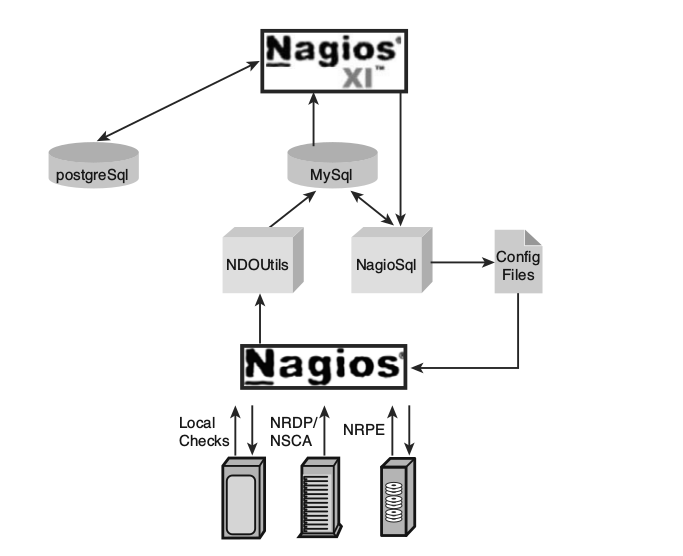
\includegraphics[width=\linewidth]{images/nagios-architecture}}
\caption{Nagios Architecture}
\label{fig:Nagios-architecture}
\end{figure}

\appendix


\end{document}
